\documentclass[12pt]{article}

% Language setting
\usepackage[english]{babel}

% Page format
\usepackage[a4paper]{geometry}
\linespread{1.5} 

% Header
\usepackage{fancyhdr}
\addtolength{\headheight}{1.5cm} % make more space for the header
\pagestyle{fancyplain} % use fancy for all pages except chapter start
\fancyhf{} % clear header text chapter
\rhead{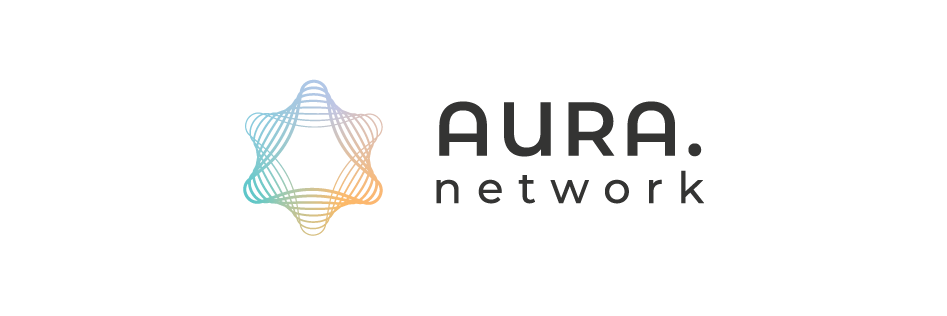
\includegraphics[height=1.3cm]{img/logo.png}} % right logo
\rfoot{\thepage}
\renewcommand{\headrulewidth}{0pt} % remove rule below header

% Useful packages
\usepackage{amsmath}
\usepackage{graphicx}
\usepackage[colorlinks=true, allcolors=blue]{hyperref}
\usepackage{draftwatermark}
\usepackage[table,xcdraw]{xcolor}

% Fix too long hyperlinks in bibliography
\usepackage{url}
\def\UrlBreaks{\do\/\do-}

\begin{document}
\title{Aura Network: a modern NFT-centric blockchain platform}
\author{admin@aura.network}
\date{\today}
\maketitle

% \begin{abstract}
% Your abstract.
% \end{abstract}

This paper gives a brief overview of \emph{Aura Network}, a layer-1 NFT-centric blockchain platform built using Cosmos SDK. Please be noted that this is an ongoing draft version that encapsulates our visi on of the network and how we are going to build it.

\section{Context}

Cryptocurrencies (crypto) are becoming more and more popular by the day. Since the birth of Bitcoin in 2009, the crypto market has grown to thousands of billions of US dollars in size. The success of crypto projects brings more innovations to the blockchain ecosystem. Recently, the hot topic of Non-Fungible Token (NFT) is an ideal case study of how blockchain technology is changing the world.

\subsection{NFT overview}
NFT origin can be traced back to the ERC-721 Ethereum token standard \cite{entriken2018erc}. An NFT is a distinguishable token that can be owned and transacted by individuals. 
Given an asset, either digitized or physical, we can issue an NFT that embeds the asset metadata including name, description, and images to represent the ownership of the NFT creator to such asset. As this ownership relation can be freely traded in the market and the unique property of the token, NFT investment is becoming widely popular. By the last quarter of 2021, the NFT sales worldwide have surged to \$ 10.5 Billion \cite{nftsale}. Among the popularity of NFT, there are 6 main categories:

\begin{enumerate}
\item Collectibles: Because NFTs are unique, possession of special NFTs is a natural demand for collectors. Some of the most well-known NFT collectibles are CryptoPunks \cite{cryptopunks}, Bored Ape Yacht Club \cite{bayc}. Any NFT can be considered collectibles. However, some have other usages in other categories as well. Currently, collectibles market value is at \$ 5.7 Billion, accounting for more than half of the whole NFT market.
\item Game: In-game assets can be represented as NFT. This unique interaction enables a new decentralized gaming trend of "play-to-earn" where players can obtain NFTs from the game then later sell them on the crypto market. Since May 2021, the Pokemon-inspired crypto game Axie Infinity \cite{axie} has rapidly gained attraction and currently provides one of the most valuable NFT collections in the world.
\item Art: Another form of collectibles NFT is digital art. NFT provides a new way for artists to increase the digital art value as it is truly unique. While the product itself can be easily copied, screen captured without permission, the origin of the art and its owner cannot. The digital artwork "Everydays: the First 5000 Days" by Beeple is a collage of 5000 images created daily by the artist in the last 13 years \cite{beeple}. The work NFT was sold for \$69 million to a crypto investor in early 2021 and is the most expensive NFT to date. Besides traditional digital arts, website likes ArtBlock \cite{artblock} provides a programmable interface to allow artists to randomly generate unique images in their respective styles and tokenize them into NFTs. 
\item DeFi: As NFT is becoming valuable, its liquidity grows. Gradually, NFT is making its way into decentralized financial solutions. nftfi \cite {nftfi} offers a platform for NFT collateralise loans. Some NFT games like Cometh \cite{cometh} intelligently integrate token swap inside the token economy and gain a lot of attraction from the crypto community.  
\item Metaverse: with the rise of NFT and the recent announcements of big tech companies like Meta \cite{facebook}, Microsoft \cite{microsoft}, Metaverse NFT has gradually become the new trend of the crypto community. Pioneer projects such as Decentraland \cite{decentraland} and The Sandbox \cite{sandbox} allow users to create and share their 3D objects. These objects can be avatars, animals, land, real estate, etc. 
\item Other Utility: Outside of gaming, NFT can also be used for other utility purposes. Using Domain names NFT services like Ethereum Name Service \cite{ens}, users can register for ``.eth" Internet domains. VeeFriends \cite{vee} from Gary Vaynerchuk allows NFT holders to join Veecon, an exclusive conference for the Gary community.
\end{enumerate}

\begin{figure}[ht]
\label{fig:nftsale}
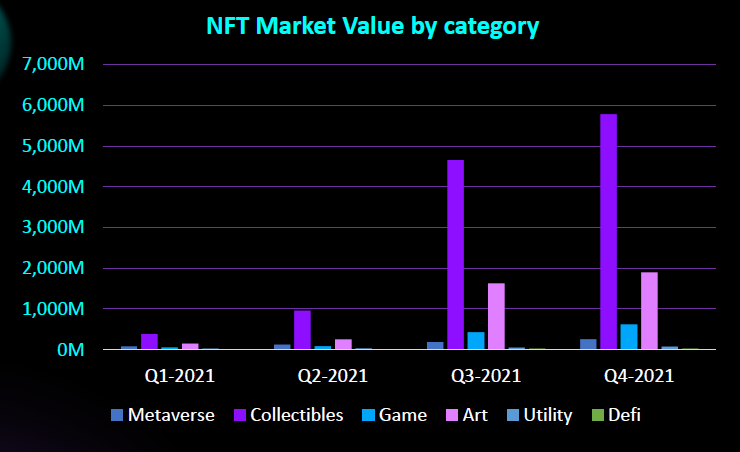
\includegraphics[width=14cm]{img/nftchart.png}
\centering
\caption{NFT Market value by categories in 2021 \cite{nftsale}}
\end{figure}

Figure \ref{fig:nftsale} shows the sale value of NFT in 2021 by these categories. We can see that most of the market value are collectibles (\$ 5.7 Billion) and arts (\$ 1.9 Billion). While this is a good sign to show the appreciation for NFT and the accessibility of the technology, we can expect more use cases for NFT in the future. NFT enables scarcity, uniqueness, and proof of ownership to any unique asset in a decentralized way, not only digital items. Thus, they can be used to pretty much anything in the world, even in the physical world. 

\subsection{Challenges}
What will the future look like for NFT? The technology is growing beyond simple collectibles or arts towards a much more diverse use of NFTs in finance, gaming, real estate, metaverse, etc. Every asset, digital or physical, can have its unique representation in the decentralized blockchain ecosystem and can be transacted without restriction. However, to enable that future, we will have to overcome several key challenges with the technology: usability, regulation, and interoperability.

\emph{Usability} is a key factor to almost all software products that end-users interact with. While NFT is just a token standard, the actual NFT object is owned, transacted by end-users through various decentralized applications (DApps). Most of the current NFT schemes are based on Ethereum, thus they inherit drawbacks from the Ethereum network as well. The confirmation time is slow, Ethereum 1 has around 15-30 transactions per second (TPS), which is extremely slow for global scale DApps. Gas price is also extremely high, especially when minting new NFTs or uploading metadata to the blockchain. Ethereum 1 carbon footprint is also very high due to the use of proof-of-work algorithm. These problems limit the utility of NFTs to use cases that concern only high-value items rather than for everything. The tech community has been working actively on this problem for years. Ethereum 2 upgrade promises a more scalable and sustainable ecosystem. However, it is still a long way until all the upgrades are in place. Alternatively, other blockchains with much better usability emerge. Flow is a new blockchain platform, originated from developers who built created CryptoKitties. Flow focuses on applications, games, and digital assets. Binance Smart Chain (BSC) also supports NFT through the BEP-721 token standard. While non of the alternative choices is as popular as Ethereum, these blockchain platforms offer a much better user experience and are more suitable for different use cases. 

Similar to any cryptocurrency scheme, \emph{regulation} is another major concern of NFT. Legally speaking, not all countries support the use and trade of NFT. Owning an NFT does not explicitly grant the owner any copyright or lawful enforcement over the real asset. Thus, investing serious tokens in NFT is not as easy as it looks. For assets like books, arts, real-life assets are taxable properties while their NFTs are not. It is unclear in the future whether NFT or any profit from NFT trading can be taxed or not.

Finally, there is little interoperability among different NFT ecosystems. There is currently no way to directly transmit an NFT from Ethereum to BSC yet. While cross-chain communications are blooming, it is still some time before we can see all of these advancements work with NFT. While the major NFT schemes are concentrated in Ethereum, this problem prevents the wide adoption of the technology to other blockchain platforms.

\section{Introducing Aura Network}
Given all of the challenges above, we introduce \emph{Aura Network}, an NFT-centric blockchain platform that focuses on expanding the use of NFT across various industries. Our vision is to create a one-stop destination for minting, evaluating, querying, and transacting NFT, to become a pioneer NFT infrastructure for the future. Aura Network focuses on solving the 3 challenges of \emph{usability}, \emph{regulation}, and \emph{interoperability} of the current NFT market.

This section provides a high-level view of 3 main aspects of Aura Network: a universal framework for managing NFT, a multi-chain solution to expand the use of NFT, and an NFT infrastructure for the metaverse.

\subsection{A universal framework for NFT}
The original token standard ERC-721 and ERC-1155 laid a foundation for NFT standard interfaces. How these tokens are created and used in DApps is not standardized. This allows developers to have more room for creativity. Wang et al. \cite{wang2021non} summarized two popular protocols for managing NFT in DApps:
\begin{enumerate}
\item \textbf{Top to Bottom:} where an owner creates the asset, mints the NFT token that represent the asset, and trades it with others through the $transferFrom$ function. This pattern is used in CryptoPunks \cite{cryptopunks}, Beeple's Everydays \cite{beeple}, etc.
\item \textbf{Bottom to Top:} where the DApp creates an NFT template that allows users to invoke and create their own unique NFT based on that template. This is used in platform-generated NFT such as Artblock \cite{artblock} and NFT games like Axie Infinity \cite{axie}.
\end{enumerate}

Most of the functions from these two protocols are concerning either the NFT creator or buyer. There might be other stakeholders in the protocol such as the DApp creator and the exchange marketplace. These are suitable for simple digital items and simple use cases. However, if we are targeting a vastly broad NFT market that involves not only collectibles and digital items but also physical assets, comprehensive digital contracts, etc., there are more parties involved. We now give an example of possible important stakeholders that may appear in such a market:

\begin{enumerate}
    \item \textbf{Custodian:} Similar to the term in banking, a custodian bank is a financial service provider that holds customers' assets for safekeeping. While "Not your keys, not your coins" is widely accepted in the blockchain community, Coinbase and various banks around the world are offering high-quality custodian services for crypto assets. They provide cold storage, security controls, and even insurance plan for protecting cryptocurrencies. This practice is also long-established for physical assets as well. Keeping authorized papers, wills or high-value items like jewels, antiques are very common for custodian services.
    
    To NFT users, custodians can offer safekeeping physical items in their safe vaults and only allow the user to redeem those items if they own the NFT. If NFT provides a way to prove the ownership of an asset, we can also expect custodians to prove that they are, indeed, holding the corresponding physical item in their safe vaults by an on-chain transaction.
    
    \item \textbf{Auditor:} In finance, an auditor refers to the person that is authorized to verify the correctness of financial documents and whether they comply with the regulation. In security, auditors conduct reviews and make sure the system is protected from common threats. In a lot of cases, the asset owner, buyer or, the exchange do a part of the auditor's job such as KYC, proving the legitimacy of papers with records, bills, etc. However, in the case of issuing NFT for high-value items like real estate, having a third-party auditor brought in to certify the legitimacy of the asset, as well as the right to sell of the owner will definitely increase the trust of the buyer and value of the item.
    
    \item \textbf{Evaluator:} In the real estate industry, property or land valuation is often a required procedure to give an estimation of market value to the property. Diamonds are evaluated based on their quality factors in clarity, color, cut, and Carat Weight. The valuation process is mostly conducted professionally and can give a relatively correct value of an asset rather than a subjective opinion. Similarly, NFTs of valuable assets can also be evaluated in a lot of criteria: the origin of the asset, level of granted permission, the market price of similar items, or depending on the utility of the NFT.
    
    \item \textbf{Asset Manager:} With items that have a high utility such as cars, real estate, a local manager who keeps track of utility usage of the item greatly benefits the community. Real estate companies often have house managing companies to do house maintenance, screen tenants, or collect rents. If NFT can represent the ownership of a building, the NFT owner not only should have all documentation relating to the properties but also can get local asset managers on board to do all the manual work for them later on. 
    
    \item \textbf{Investor:} Another new use case of NFT is to fractionize the NFT to allow multiple investors to co-invest in the item. This fractional ownership adds new ways for integrating NFT with DeFi schemes such as Uniswap as each fraction is fungible. Thus, multiple investors can pool up and join the NFT investment game.
\end{enumerate}

Custodian, auditor, evaluator, asset manager, and investors are just some samples of possible stakeholders that are needed in the NFT market. We have seen some use cases that require those parties. However, a complete platform that allows all of them to work together on-chain is unheard of. This is why we create Aura Network. We envisioned Aura Network to be a one-stop destination for all stakeholders and projects in the NFT ecosystem. Every interaction with NFT and its counterpart in the physical world should be reflected on-chain.

\subsection{Connecting to other Blockchains}

With the success of Bitcoin, Ethereum, Cardano, and others, a lot of crypto project was born, creating many isolated blockchain networks. With multiple blockchains coexisting, cross-chain communication solutions emerge. Atomic swap, cross chain messages are all examples of the capability to link different blockchains together to create a more cohesive ecosystem that benefits everyone. However, at the moment, there is not yet a mainstream solution for either moving an NFT from one blockchain to another, or having multiple NFT on multiple blockchains that represent the same asset. While this is mostly due to the poor interoperability among different blockchain platforms, we can expect that this issue can be resolved in the near future due to the advancement of cross-chain bridges similar to XP.Network \cite{xpnetwork} or related projects. 

Another part of blockchain community that we need to look at is the private blockchain sector. Standing beside the success of crypto projects, private blockchain projects are slowly gaining attractions. Private, consortium or permissioned blockchain often refer to systems that consist of one or several authorized parties that create a blockchain network for specific business purposes. Imagine a group of companies who want to create a distributed network for transparently exchanging assets, tracking items or sharing documents. Unlike its counterpart, private blockchain is more appealing for companies, enterprises or governments as they are easier to control and do not require volatile currencies to operate. Success of the crypto trend in 2020 also brought a lot of opportunities to private blockchain eco-system. The private blockchain sector is predicted to generate \$176 Billion in 2025 then surge to  \$ 3.1 Trillion in business value by 2030 \cite{privatebc}. 

Can NFT become a game changing use case in private blockchain ? a lot of businesses are looking into loyalty, insurance or traceability use cases where the blockchain ledger is an immutable storage of important data. This fits the idea of NFT very well. However, there isn't any mainstream use case that can bring NFT to the private blockchain sector. Typically, enterprises or businesses are main adopters of private blockchain as they  require more control over the network. By having a bridge to public blockchain and vice versa, NFTs defined on Ethereum, BSC and other networks can be moved to private chains, where they have more utility in dealing with real world problems that businesses are dealing with in their private blockchain setup. In turn, by having a route to the public side, businesses now have access to a market of millions users and billions USD worth of values circulating every day. This increases liquidity on private networks massively and enables many other use cases that a single blockchain network can not achieve.

This is the second aspect that Aura Network is trying to solve. The Aura blockchain platform should be capable of bridging to other blockchain network, either public or private ones and vice versa. Thus, NFT owners can bring their on0chain assets to any place, any app, at any time. 

\subsection{Towards the metaverse}
In this last section, we look at the recently popular trend of ``metaverse". The word is a combination of ``meta" and ``universe". It describes a hypothetical virtual world that is linked to the physical world. The term was coined in a science fiction novel \emph{Snow Crash} by Neal Stephenson in 1992. While the concept of virtual world is not new as computer games has been around for decades, the metaverse concept brings more integration between virtual and physical world. In the metaverse, users are represented as \emph{Avatars} and through them, they can interact with the digital environment which is a metaphor of the real world \cite{lee2021all}.

While the term \emph{metaverse} was coined in 1992, the development of the idea was dated way before it. The table top game \emph{Dungeon \& Dragons} was published in 1974, allowing players to submerge in a fantasy medieval European theme world with super powers and mythical creatures. That was more than a decade when the first personal computer was introduced. Later on, with the booming of the Internet, the table top imaginative world then become virtual, digital world of massively multiplayer online games (MMOG) such as \emph{Second Life}, \emph{Minecraft}. Players then can also have a mix experience of the virtual and physical world through games like \emph{Pokemon Go} and extended reality hardware devices like \emph{Hololens} or \emph{Oculus Rift}. Blockchain based Metaverse came later. The NFT game \emph{Crypto Kitties} in 2017 is the first popular blockchain game that allows players to truly own in-game assets and create a new blockchain based virtual economy. Following the kitties, other games like \emph{Decentraland}, \emph{The Sandbox}, etc. are creating new opportunities for players to not only submerge into the metaverse world, but also actually own some part of it themselves.

The metaverse is more than just games. Lee et al \cite{lee2021all} show us the three steps of evolution in technology that support metaverse. The first step of \emph{Digital Twins} is where physical objects can be projected to their digital form. Photos, 3D models are the examples. Next step is \emph{Digital Natives} where users can freely create new content, virtual object that are based on the projected ones. User can own it, sell it in a decentralized manner, etc. This is already achieved in NFT games. Finally the last one, \emph{Co-existence} is where both physical and digital objects exists, are linked together and users can interact with both. This is the step that Aura Network wants to aim for.   

\begin{figure}[ht]
\label{fig:metaverse}
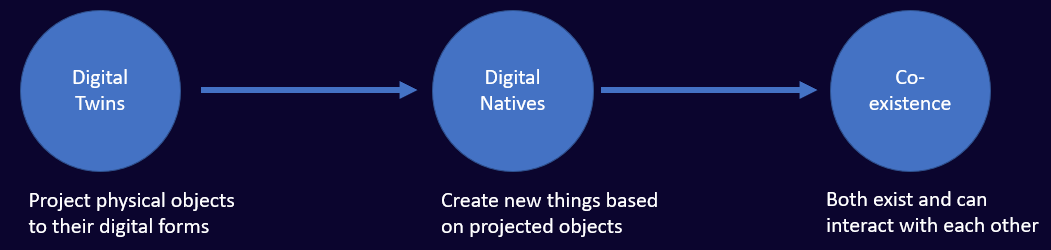
\includegraphics[width=14cm]{img/metaverse.png}
\centering
\caption{Evolution states of metaverse \cite{lee2021all}}
\end{figure}

Mapping real world, physical asset to NFT is an important step in achieving the co-existence state of the metaverse. As an universal framework for working with NFT, Aura Network final step is to work with games and service providers like Decentraland, Axie Infity, Meta, Microsoft, etc. to bring NFT on chain to these virtual world.

\section{Architecture}
In this section, we will present the high level software architecture of the Aura Network ecosystem. Particularly, we will first go through the architecture of the Aura Blockchain platform. Next is the envisioned eco-system that we will build on top of the platform and finally, we give an overview of a complete hypothetical use case of mapping real life assets on the Aura Network.

\subsection{Blockchain Platform}
The Aura Network Blockchain platform is a \emph{Layer-1 blockchain} built using \emph{Cosmos SDK} \cite{kwon2019cosmos}. The Cosmos SDK is an open-source framework for building proof-of-stake blockchains. It allow developers to create a blockchain platform from scratch with native interoperate capability with other blockchain platforms. 

\begin{figure}[ht]
\label{fig:architecture}
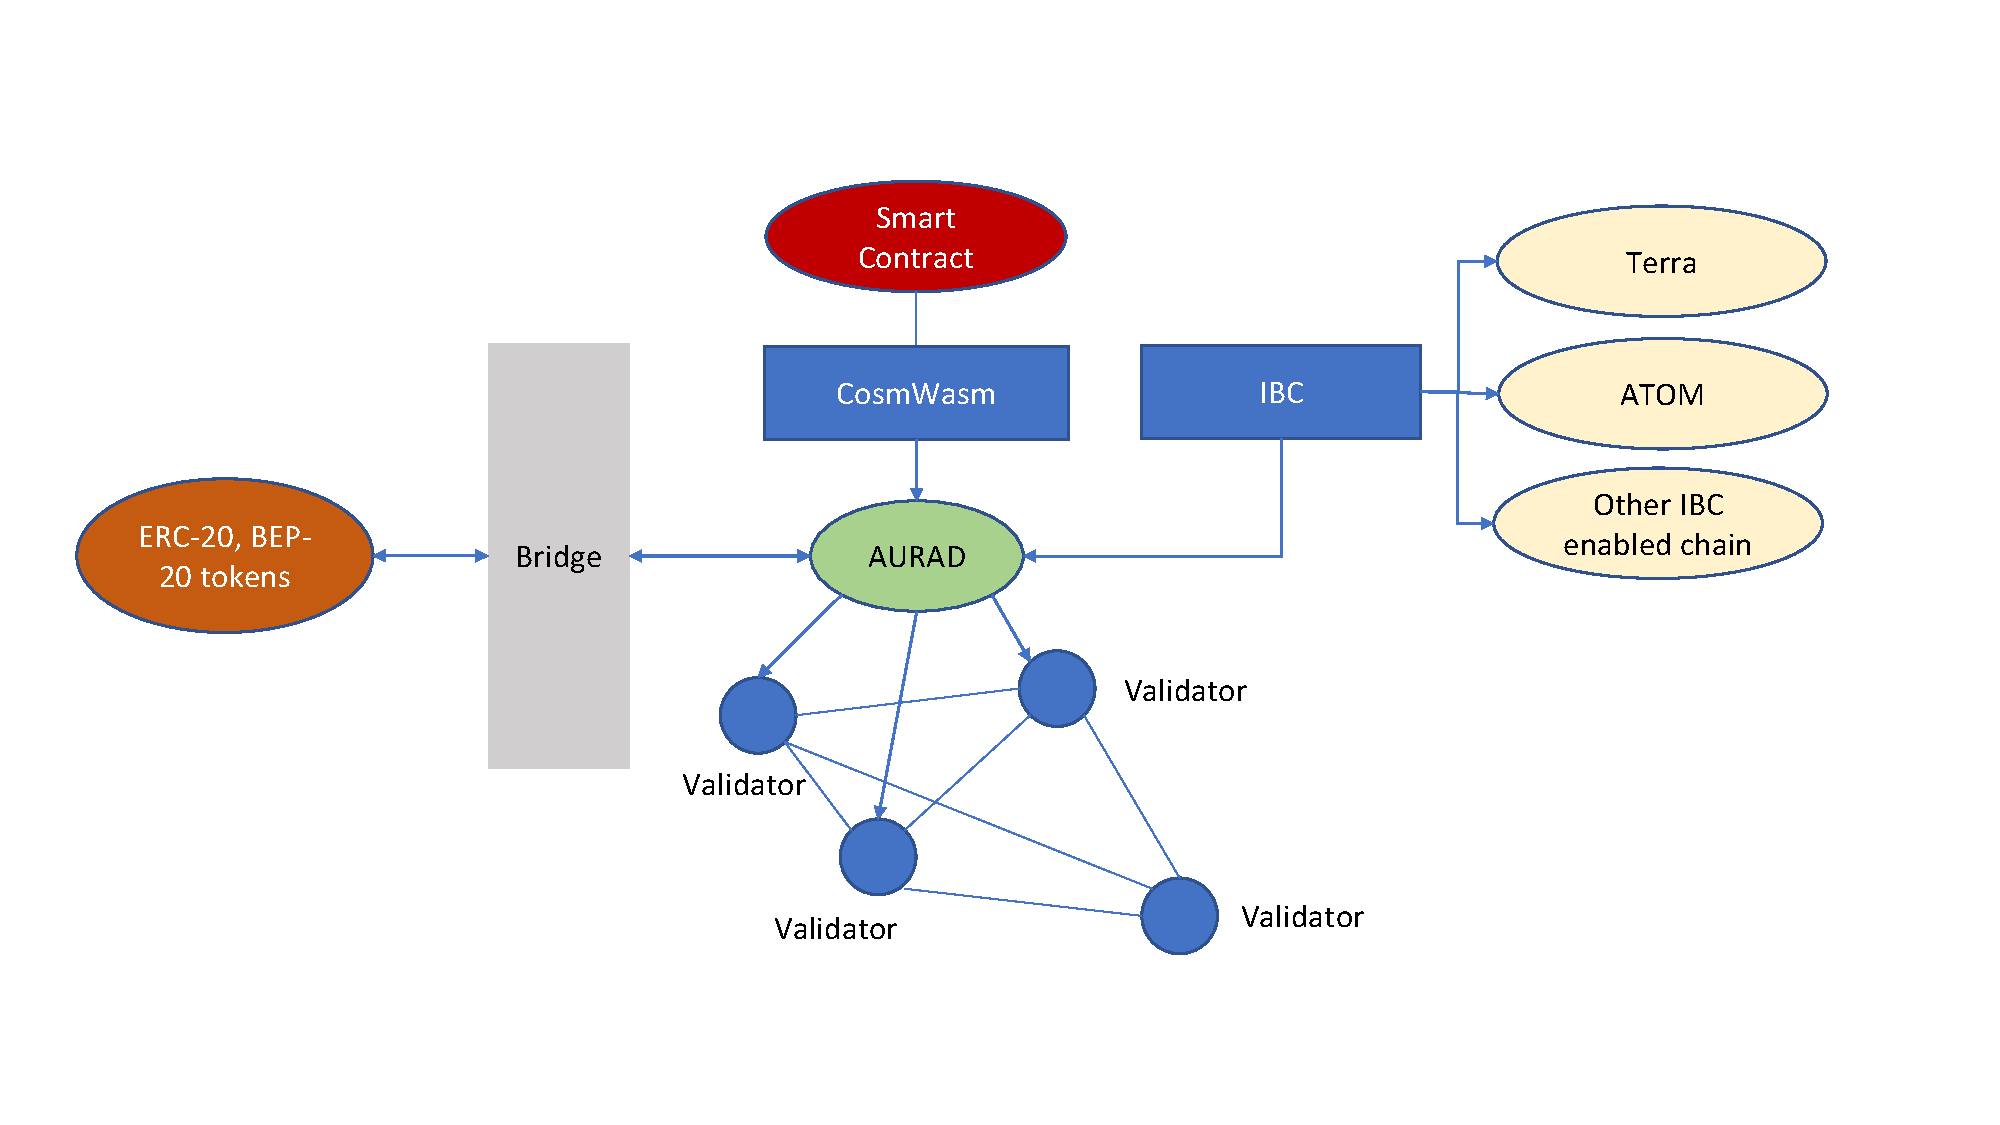
\includegraphics[width=\textwidth, trim={5cm 2cm 5cm 0}, clip]{img/architecture.pdf}
\centering
\caption{The Aura Network blockchain platform architecture}
\end{figure}

Figure \ref{fig:architecture} shows the high level architecture of the Aura blockchain platform. There are several main components that we want to highlight in this architecture:

\subsubsection*{Validator}
\emph{Validators} are blockchain nodes that participate in the consensus process to confirm transactions and producing blocks.
The consensus engine is \emph{Tendermint}~\cite{buchman2016tendermint}, a Byzantine Fault Tolerance state machine replication engine while he Proof-of-Stake (PoS) logic layer is provided by the Cosmos SDK. 

\subsubsection*{aurad}
\emph{aurad}, short form of ``Aura Daemon" refers to the compiled platform binary that runs on all Validator nodes. aurad contains standard Cosmos modules like \emph{Auth}, \emph{Bank}, \emph{Mint}, \emph{Slash}, \emph{Stake}, etc.that are required to run the blockchain platform. There are a few simple modifications such as adding parameters and specific business logic that may be required by the Aura tokenomics. But overall, there won't be much change from the provided modules from Cosmos.

\subsubsection*{CosmWasm}
CosmWasm stands for ``Cosmos WebAssembly", it's a Cosmos module that enables WebAssembly virtual machines in the cosmos SDK. As the smart contract written for CosmWasm is compatible with all other blockchain based on Cosmos, we choose CosmWasm as the middleware for building smart contracts and DApps for the Aura ecosystem. Currently it only support contract written in \emph{Rust}, but many high level programming languages can be added in the future.

\subsubsection*{Bridge}
Bridge is also an important part of aurad. As Aura Network focuses on bridging assets to other blockchains even outside of the Cosmos SDK, bridge modules that support  Inter-Blockchain Communication Protocol (IBC) are the best way of doing this. Currently, there is already \emph{Gravity} bridge that connect Cosmos-based blockchain to Ethereum. We also see that IBC bridge is in development for other blockchains, including private ones like Hyperledger Fabri, a more popular choices for building consortium blockchain in enterprises. 

\subsection{Aura Network ecosystem}
Figure~\ref{fig:architecture} shows the potential building blocks of the Aura Network. At the moment, we divide the ecosystem into 6 main categories

\begin{figure}[ht]
\label{fig:auraeco}
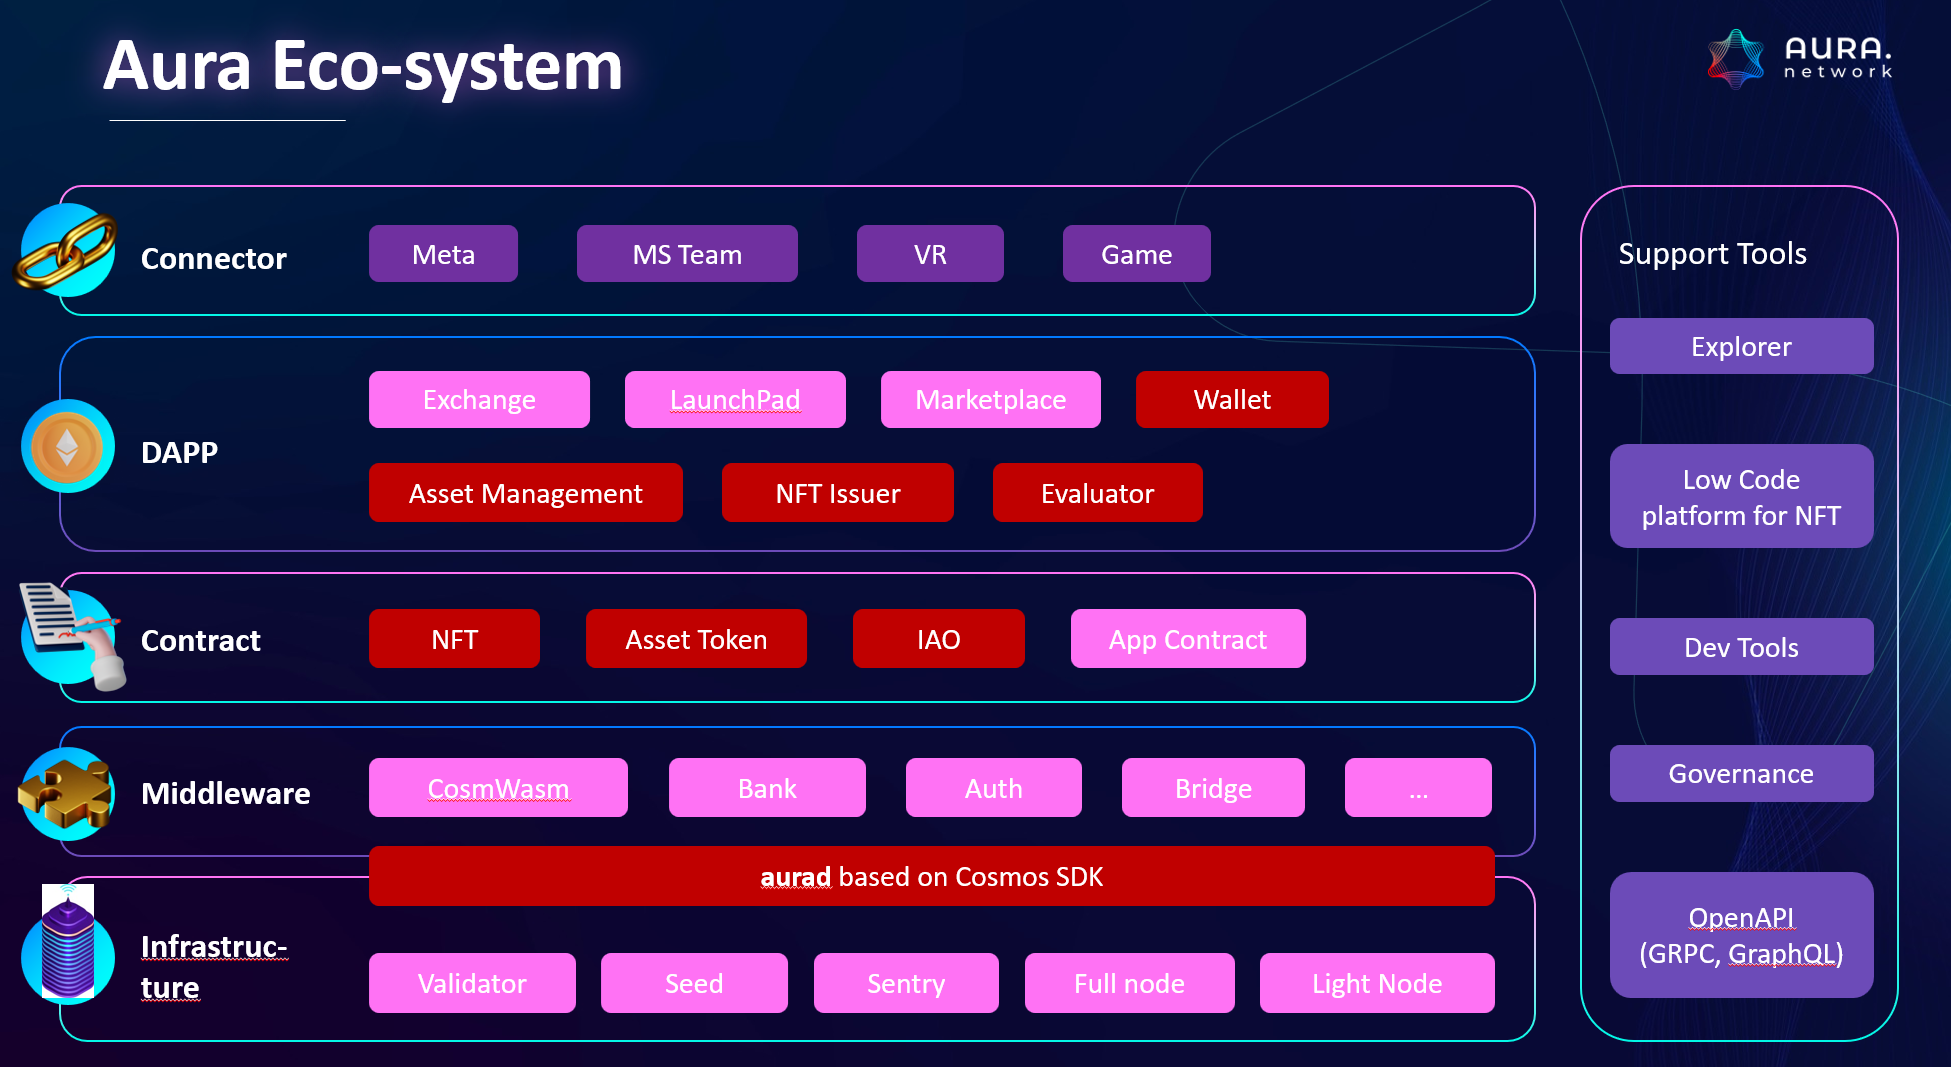
\includegraphics[width=14cm]{img/auraeco.png}
\centering
\caption{The Aura eco-system}
\end{figure}

\subsubsection*{Infrastructure}
The Infrastructure layer mostly refers to the blockchain platform that is mentioned above. Other than validators, Cosmos and Tendermint best practices in running production software also include Seed, Sentry, Full and Light node. Details on the setup of these nodes are described in the Cosmos SDK documentation. We will also provide scripts and instruction on how to setup different types of node later on through Aura development documents.

\subsubsection*{Middleware}
The middleware layer contains Cosmos modules bundled together with aurad. As mentioned, most of the provided Cosmos modules are included. The Aura team also publishes modification to these modules in the development docs as well.

\subsubsection*{Smart Contract}
Smart contract layer contains smart contracts written in Rust, compiled and ran on the CosmWasm module.

\subsubsection*{Decentralized App}
Decentralized Applications (DApps) are the main focus of the Aura Network. All business solutions are written here such as: NFT Asset Management, Wallet, NFT Issuer, NFT evaluation, Exchange, Launchpad, Marketplace, etc. As Aura Network focuses on NFT businesses, the Aura team will take the lead in developing these DApps to attract all types of stakeholders as mentioned in the introduction section.

\subsubsection*{Connector}
Connector layer contains integration APIs, SDKs that are used to bring NFT assets to Metaverse networks. By itself, Aura Network does not provide a metaverse experience, but to provide infrastructures for bringing NFT assets to the metaverse.

\subsubsection*{Support Tools}
This layer contains usual software tools that are mandatory to the Aura blockchain platform. That contains blockchain explorer, low code software development, development tools, OpenAPI and Governance tools.

\section{Tokenomics}

This section describes information related to native currency supported by the Aura Network.

\subsection{Token Usage}
We introduce 2 types of native tokens in the Aura Network: the Aura Token on Ethereum and Aura Coin. Both actually refers to the same unit.

\begin{enumerate}
    \item Aura Token on ETH: To launch Aura Network, we first introduce the ERC-20 Aura Token on Ethereum. This token only acts as a place holder for the later Aura Coin that will be introduced when Aura Mainnet launches. Like other ERC-20 tokens, Aura Token can be traded on the cryptocurrency market until Aura Coin is introduced.
    \item Aura Coin: Aura Coin is the native currency of the Aura Network blockchain platform. Besides the trading capability of Aura Token, Aura Coin has many other utilities:

    \textbf{Staking}: Aura Coin holder can delegate their coins to trusted validators to earn passive commission income from the network.
    
    \textbf{Governing}: Aura Coin holder can participate in voting for software updates or other important decisions of how the Aura community should be developed.
    
    \textbf{Transaction fee}: Aura Coin is used to pay for transaction fee.
    
    \textbf{Exchange and Swap}: Aura Coin can be exchange or swap in the market
    
    \textbf{Payment for Utility Services}: As Aura focuses on bringing real world assets and different stakeholders to the ecosystem to offer business services, Aura Coin can be used for payment for these utility services. Aura holders can vote to choose their service providers (evaluator, auditor, etc.) and use Aura to pay for their services.
\end{enumerate}

As the Aura Token is just a temporary placeholder for the Aura coin, we expect a transition period where one can ``convert" their token on ETH to receive their corresponding amount of Aura coin on the Aura main network. After receiving Aura coin, Aura Token will be burnt.

\subsection{Token Distribution}
% Please add the following required packages to your document preamble:
% \usepackage{graphicx}
% \usepackage[table,xcdraw]{xcolor}
% If you use beamer only pass "xcolor=table" option, i.e. \documentclass[xcolor=table]{beamer}
\begin{table}[ht]
\label{table:tokenomics}
\centering
\resizebox{\textwidth}{!}{%
\begin{tabular}{|l|l|l|l|l|}
\hline
\rowcolor[HTML]{343434} 
{\color[HTML]{FFFFFF} Token Allocation} & {\color[HTML]{FFFFFF} Allocation (\%)} & {\color[HTML]{FFFFFF} AURA} & {\color[HTML]{FFFFFF} TGE (\%)} & {\color[HTML]{FFFFFF} Vesting Schedule (monthly)}          \\ \hline
Ecosystem Growth                        & 20                                     & 200M                        & 50                              & Linear vesting over 2 years                      \\ \hline
Strategic                               & 20                                     & 200M                        & 0                               & Linear vesting over 2 years                      \\ \hline
Public Distribution                     & 5                                      & 50M                         & 100                             & No vesting                                       \\ \hline
Foundation Reserves                     & 10                                     & 100M                        & 0                               & Linear vesting over 2 years                      \\ \hline
Team                                    & 20                                     & 200M                        & 0                               & 1 year cliff then linear vesting   over 3 years  \\ \hline
Block Rewards                           & 25                                     & 250M                        & 0                               & Rewards   for validator per block over 10 years. \\ \hline
\end{tabular}%
}
\caption{Aura token distribution design}
\end{table}

Table~\ref{table:tokenomics} shows the token distribution metrics for Aura Network. The maximum amount of Aura can be minted is exact \textbf{1 Billion} tokens. This value is specified in the Aura genesis block and cannot be changed in the future unless we do a hard fork. This is applied for both Aura Token on ETH and the Aura Coin as the token is simply just a placeholder.

There are 6 categories that Aura coin will be allocated to:
\begin{enumerate}
    \item \textbf{Ecosystem Growth}: 20 percents of the total coin will be allocated to ecosystem growth fund. This fund is used for ecosystem development such as project grant, bug bounties, attracting stakeholders to provide utility services, etc. 
    \item \textbf{Strategic investment}: 20 percents of the total coin go to private sales for strategic partners.
    \item \textbf{Public Distribution}: 5 percents of the total coin will go to Aura Initial Exchange Offering for public sale.
    \item \textbf{Foundation Reserve}: 10 percent of the total coin will be stored in the foundation treasury fund. All decisions on how to spend the fund must go through public governance process by Aura coin holders. 
    \item \textbf{Team}: 20 percents of the total coin will go to the Aura team.
    \item \textbf{Block Rewards}: 25 percents of the total coins will be periodically minted as block rewards to distribute to validators.
\end{enumerate}

\subsubsection{Token generation event}
There are 2 \emph{Token Generation Events} (TGE) that are corresponding to the 2 types of native currency in the network, the token and the coin. For Aura Token on Ethereum, the token generation is quite standard as the Aura team will mint and transfer tokens manually based on the specification in table~\ref{table:tokenomics}.

By the time of Aura Mainnet release and the listing of Aura Coin, the Aura Token contract on ETH will be frozen so that no more token can be minted. Aura Token holders then can claim their coins on the Aura Mainnet by sending their tokens on ETH to the migration contract. These tokens can be burnt later on. The state of vesting schedule at the time will also be replicated to the Mainnet. 

\subsubsection{Account Vesting}
Vesting refers to the process of locking a certain amount of coins or tokens then gradually release them with time. Other than public distribution coins, the rest of the token allocation categories are locked and vested on different terms. Similar to TGE, vesting Aura tokens or coins are different.


\subsubsection{Block Rewards}

\section{Roadmap}

\section{Conclusion}

\bibliographystyle{plain}
\bibliography{references}

\end{document}